\documentclass[a4paper]{article}

\usepackage[swedish]{babel}
\usepackage[latin1]{inputenc}
\usepackage{geometry}
\usepackage{amssymb}
\usepackage{framed}
\usepackage{amsmath}
\usepackage{graphicx}
\usepackage{booktabs}
\usepackage{subcaption}

\setlength{\parindent}{0pt}
\setlength{\parskip}{3ex}

\begin{document}

\begin{center}
  {\large Artificial Neural Networks and Deep Architectures, DD2437}\\
  \vspace{7mm}
  {\huge Short report on lab assignment 2\\[1ex]}
  {\Large Radial basis functions, competitive learning and self-organisation}\\
  \vspace{8mm}  
  {\Large Hilding Wollbo\\}
  \vspace{4mm}
  {\large September 20, 2020\\}
\end{center}

%\begin{framed}
%Please be aware of the constraints for this document. The main intention here is that you learn how to select and organise the most relevant information into a concise and coherent report. The upper limit for the number of pages is 6 with fonts and margins comparable to those in this template and no appendices are allowed. \\
%These short reports should be submitted to Canvas by the authors as a team before the lab presentation is made. To claim bonus points the authors should uploaded their short report a day before the bonus point deadline. The report can serve as a support for your lab presentation, though you may put emphasis on different aspects in your oral demonstration in the lab.
%Below you find some extra instructions in italics. Please remove them and use normal font for your text.
%\end{framed}

\section{Main objectives and scope of the assignment}

%\textit{List here a concise list of your major intended goals, what you planned to do and what you wanted to learn/what problems you were set to address or investigate, e.g.}\\
My major goals in the assignment were  
\begin{itemize}
\item to study the use and implementation of radial basis functions (RBF) with competitive learning (CL)
\item to use this architecture to perform function approximation in the presence of noise
\item to study and implement self organizing maps (SOM) for clustering of data according to similarity
\end{itemize}

%\textit{Then you can write two or three sentences about the scope, limitations and assumptions made for the lab assignment}\\

\section{Methods}
%\textit{Mention here in just a couple of sentences what tools you have used, e.g. programming/scripting environment, toolboxes. If you use some unconventional method or introduce a clearly different performance measure, you can briefly mention or define it here.}\\
The architectures and tasks in the lab were developed in python, using common libraries such as numpy for easy manipulation of vectors, generation of random samples and other mathematical operations. The pandas library was used in order to facilitate reading and manipulation of data from .dat files.
\section{Results and discussion - Part I: RBF networks and Competitive Learning \normalsize{\textit{(ca. 2.5-3 pages)}}}

%\begin{framed}
%\textit{Make effort to be \textbf{concise and to the point} in your story of what you have done, what you have observed and demonstrated, and in your responses to specific questions in the assignment. You should skip less important details and explanations. In addition, you are requested to add a \textbf{discussion} about your interpretations/predictions or other thoughts concerned with specific tasks in the assignment. This can boil down to just a few bullet points or a couple of sentences for each section of your results. \\ Overall, structure each Results section as you like. Analogously, feel free to group and combine answers to the questions, even between different experiments, e.g. with noise-free and noisy function approximation, if it makes your story easier to convey. \\
%\\Plan your sections and consider making combined figures with subplots rather than a set of separate figures. \textbf{Figures} have to condense information, e.g. there is no point showing a separate plot for generated data and then for a decision boundary, this information can be contained in a single plot. Always carefully describe the axes, legends and add meaningful captions. Keep in mind that figures serve as a support for your description of the key findings (it is like storytelling but in technical format and academic style. \\
%\\Similarly, use \textbf{tables} to group relevant results for easier communication but focus on key aspects, do not overdo it. All figures and tables attached in your report must be accompanied by captions and referred to in the text, e.g. $"$in Fig.X or Table Y one can see ....$"$. \\
%\\When you report quantities such as errors or other performanc measures, round numbers to a reasonable number of decimal digits (usually 2 or 3 max). Apart from the estimated mean values, obtained as a result of averaging over multiple simulations, always include also \textbf{the second moment}, e.g. standard deviation (S.D.). The same applies to some selected plots where \textbf{error bars} would provide valuable information, especially where conclusive comparisons are drawn.} 
%\end{framed}

\subsection{Function approximation with RBF networks\\ \normalsize{\textit{(ca. 1.5-2 pages)}}}
%\textit{Combine results and findings from RBF simulations on both noise-free and noisy function approximation (sin(2x) and square (2x)). Try to organise them into subsections, and please make sure you pay attention to the comparison between RBF- and MLP-based approaches as well as the comparative analyses of batch and on-line learning schemes. Answer the questions, quantify the outcomes, discuss your interpretations and summarise key findings as conclusions.}
\paragraph{Batch learning of network weights}
Two simple functions were chosen to be used for studying regression using RBF networks, the $\sin(2x)$ and its corresponding square function. Training and test data was generated by equally sampling the interval $[0, 2\pi]$. The RBF-units were placed uniformly in this region, which makes sense for the quite regular sine function, but might however be a suboptimal policy for estimating the sharp transitions of the square function. 
By setting the RBF-node variance to 0.5, the sine wave could readily be estimated with as little as $0.1, 0.01$ and $0.001$ absolute error using 8, 13 and 20 units respectively. For the square function, less than $0.1$ absolute error was achieved using 30 units and a narrower node variance of $0.1$. The error could be further reduced by increasing the number of nodes and making the node variance even more narrow, but for higher amounts of nodes my implementation became unstable. One simple way to achieve perfect reconstruction with zero error for the square function is to simply transform the estimated value using a sign transform. Using this method, perfect estimation of the signal could be achieved using as little as 14 units. Of course, the hardest parts of the signal to estimate are the transition points when the signal switches polarity. One application of this network could be for generating signal pulses in digital communication systems.
\\
\begin{figure}[ht]
   \begin{subfigure}[b]{0.5\textwidth}
	 \centering
	 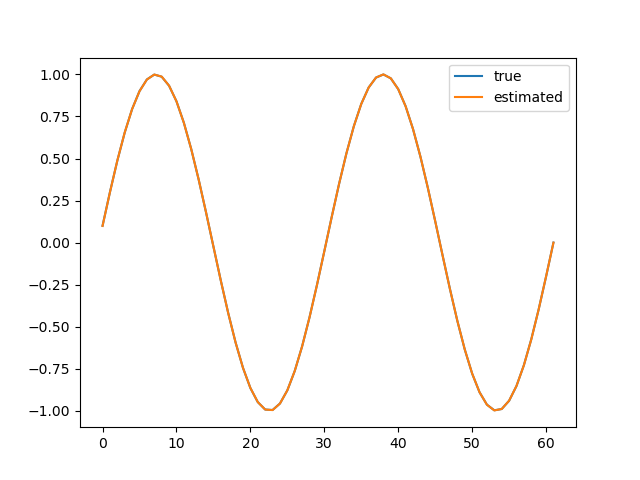
\includegraphics[width=\linewidth]{figures/sineclean.png}
   \end{subfigure}
 	\begin{subfigure}[b]{0.5\textwidth}
	 \centering
	 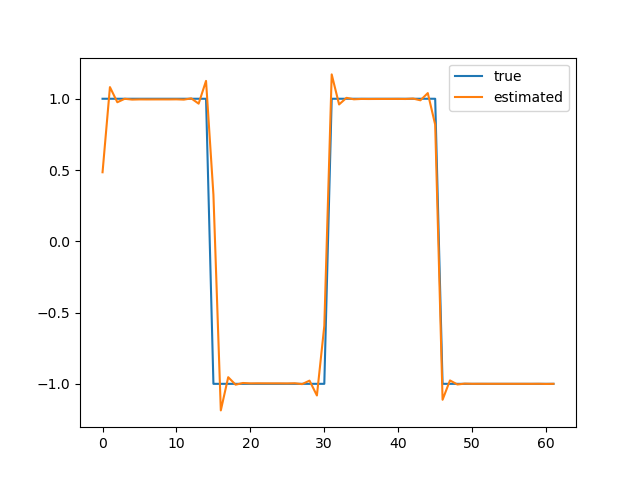
\includegraphics[width=\linewidth]{figures/squareclean.png}
   \end{subfigure}
   \caption{The estimated functions using 30 nodes.}
\end{figure}
Adding noise to the system complicates the estimation process, especially since noise is added to both training and test datasets. However, by widening the RBF-nodes, we can decrease the degree to which the system models the individual noise realisations and instead models the underlying true function. The problem with this is that the mean of the function might become slightly biased. When using the sign transform, it is important that the node variances are not set too low in order to detect the sharp transitions of the square function, since the sign transform can avoid the incurred noise.
\\
\begin{figure}[ht]
   \begin{subfigure}[b]{0.5\textwidth}
	 \centering
	 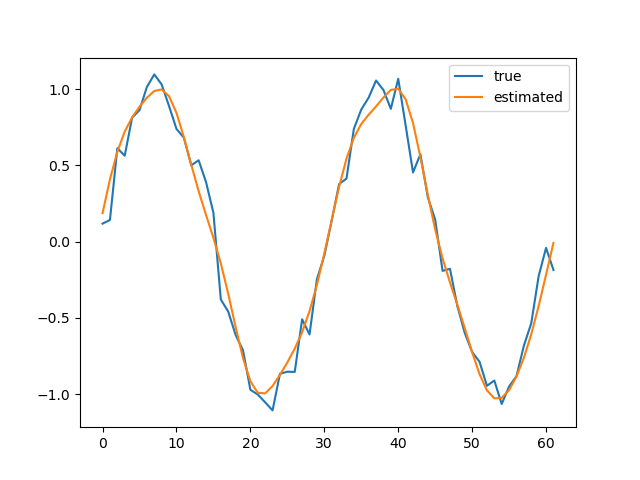
\includegraphics[width=\linewidth]{figures/sinenoisy.png}
   \end{subfigure}
 	\begin{subfigure}[b]{0.5\textwidth}
	 \centering
	 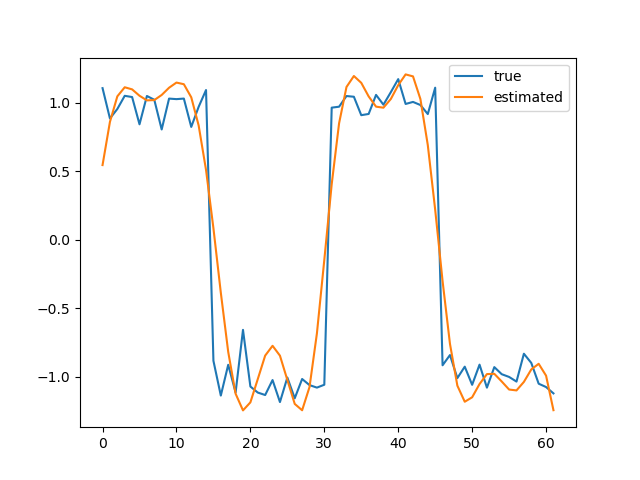
\includegraphics[width=\linewidth]{figures/squarenoisy.png}
   \end{subfigure}
   \caption{The estimated functions using 30 nodes.}
\end{figure}
Another strategy to initialize the weights for estimation of the square function was implemented by using a Gaussian Mixture Model to generate rbf-centres. The GMM centres were placed in the sharp transition points of the functions, namely $[\pi/2, \pi, 3\pi/2]$. This strategy improved the tracking of the sharp corners, but gave rise to more variance. Thus, in order to estimate the square function, it is simply better to use the sign transform than trying to estimate it directly through regression.
In general, using batch learning was computationally challenging and prone to instability since taking the inverse is very sensitive to the selected model size and variance parameters in the RBF-nodes. When adding more nodes, the overlap between the RBF-functions increase, which implies that rows in the Gram matrix become similar, which in turn leads to the determinant approaching zero and thus numerical instability. One way to remedy this is to add a very minor amount of regularizing noise to the diagonal entries of the Gram matrix, but this introduces some error to this estimation. This prompts the study of online learning methods as well.
\paragraph{Online learning of network weights}
Using online learning, we can reduce the sensitivity of the system to taking inverses of degenerate matrices. Increasing the number of RBF units increase the amplitude of the estimated function. Thus, in order to account for this, the variance of the individual RBF-nodes need to be reduced, which increases the noise of the estimated function. At the same time, we can further modify the behaviour of the estimation by manipulating the number of epochs as well as the learning rate. Increasing the learning rate and the number of nodes generally lead to an increased amplitude, while reducing the width of the RBF-nodes introduced more noise but allowed the system to detect more rapid changes. 
\begin{figure}[ht]
   \begin{subfigure}[b]{0.5\textwidth}
   \centering
   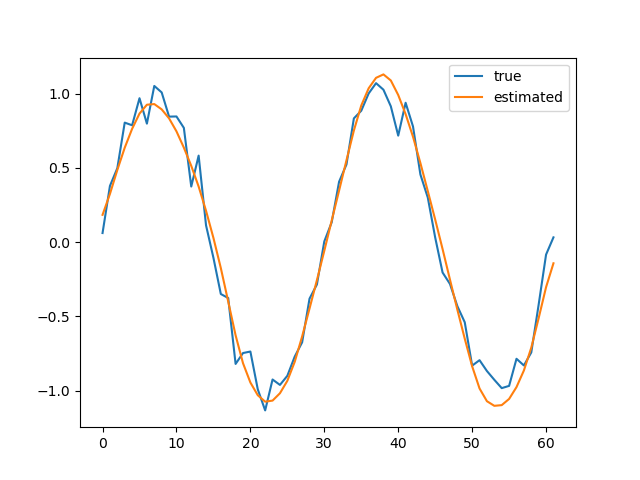
\includegraphics[width=\linewidth]{figures/sineonline.png}
   \subcaption{20 nodes, kernel width 0.2}
   \end{subfigure}
  \begin{subfigure}[b]{0.5\textwidth}
   \centering
   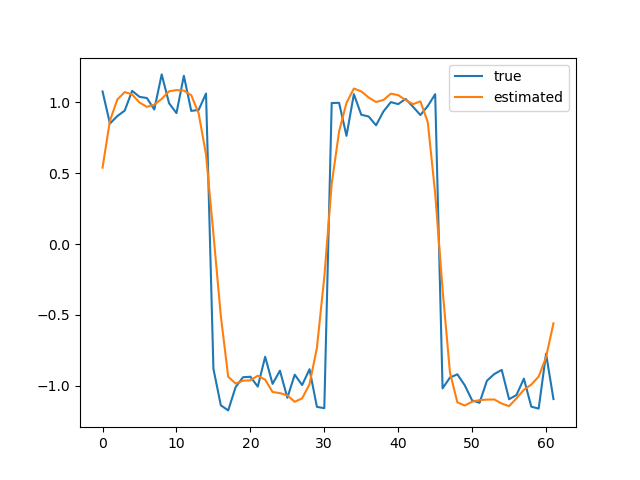
\includegraphics[width=\linewidth]{figures/squareonline.png}
   \subcaption{40 nodes, kernel width 0.09}
   \end{subfigure}
   \caption{The estimated functions using online learning over 100 epochs and $\eta$=0.01.}
\end{figure}
\subsection{Competitive learning for RBF unit initialisation\\ \normalsize{\textit{(ca. 1 page)}}}
Competitive learning (CL) was implemented to study unsupervised learning of initial RBF-unit weights for two dimensional data. The RBF-units were initially placed in an uniform grid in the input space with a slight random perturbation. The algorithm was implemented using a gaussian kernel as output basis function to measure the similarity between the winner and the other nodes. A node was selected as a winner if its distance using the gaussian kernel was smaller than a threshold $\delta$. In order to facilitate learning and avoid dead units, the width of the gaussian kernel was selected to exponentially decay for every iteration. Using four and nine RBF-units respectively, a learning rate of 0.01 and 100 epochs produced the mappings in Figure \ref{fig:cl_init}. These units condense where there are many samples, while still covering the complete input space.

\begin{figure}[ht]
   \begin{subfigure}[b]{0.5\textwidth}
   \centering
   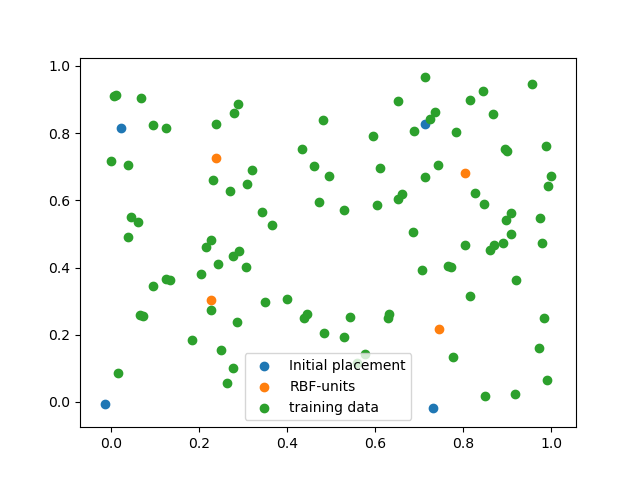
\includegraphics[width=\linewidth]{figures/RBF_cl_2.png}
   \subcaption{4 nodes.}
   \end{subfigure}
  \begin{subfigure}[b]{0.5\textwidth}
   \centering
   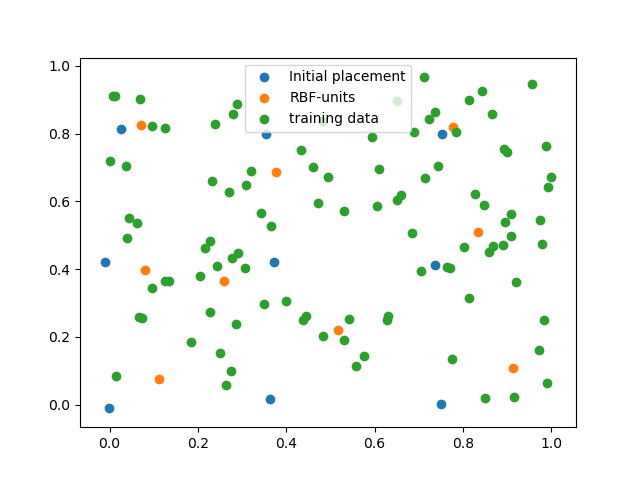
\includegraphics[width=\linewidth]{figures/RBF_cl.png}
   \subcaption{9 nodes.}
   \end{subfigure}
   \caption{The resulting initializations using 100 iterations and $\eta$=0.01.}
   \label{fig:cl_init}
\end{figure}

\section{Results and discussion - Part II: Self-organising maps \normalsize{\textit{(ca. 2 pages)}}}
To study how self organising maps may be used for unsupervised learning, three different datasets and tasks were studied.
\subsection{Topological ordering of animal species}
For this task, a SOM-network was trained to topologically sort and order a given set of animals. There were 32 animal species, each of which had 84 binary features. The network was initialized randomly with 100 x 84 entries between 0 and 1. For each animal in the set, a winning node in the matrix was selected, and it and its neighbors in the output space were updated, eventually converging to the ordering shown in \ref{tab:animals}. Similar animals are mapped together, the most abrupt transition is in my opinion 'giraffe' to 'spider', but it can be seen that they are the furthest away of every neighbouring entry when measuring by the distance in SOM-indices.

\begin{table}
\centering
\begin{tabular}{@{}llll@{}}
  \toprule
    SOM-index & Animal & SOM-index & Animal \\
  \midrule
  0   &     'kangaroo' & 52     &   'ostrich'\\
  3   &      'antelop' & 57     & 'crocodile'\\
  7   &        'horse' & 59     & 'seaturtle'\\
  10  &          'pig' & 62     &      'frog'\\
  12  &        'camel' & 66     &    'walrus'\\
  13  &      'giraffe' & 70     &       'ape'\\
  20  &       'spider' & 73     &      'bear'\\
  23  &      'moskito' & 75     &     'hyena'\\
  25  &     'housefly' & 80     &       'dog'\\
  29  &    'butterfly' & 83     &      'lion'\\
  32  &  'grasshopper' & 84     &       'cat'\\
  34  &       'beetle' & 87     &     'skunk'\\
  36  &    'dragonfly' & 90     &       'bat'\\
  42  &      'pelican' & 93     &  'elephant'\\
  45  &         'duck' & 95     &       'rat'\\
  48  &      'penguin' & 97     &    'rabbit'\\
\bottomrule
\end{tabular}
\caption{The animals sorted through the SOM-algorithm.}
\label{tab:animals}
\end{table}
\subsection{Cyclic tour}
The same SOM-algorithm was implemented for the task of mapping the nodes from a 2-D input space to a closed curve in 1-D. The dataset consisted of 10 city positions in 2-D, and the network was trained for 10 output nodes. These nodes were then trained to map the cities, and each city was assigned a closest RBF-node. Through this implementation, we can find a loop through the cities by mapping a curve through the cities by their RBF-neighbours, shown in Figure \ref{fig:cities}

\begin{figure}[ht]
   \begin{subfigure}[b]{0.5\textwidth}
   \centering
   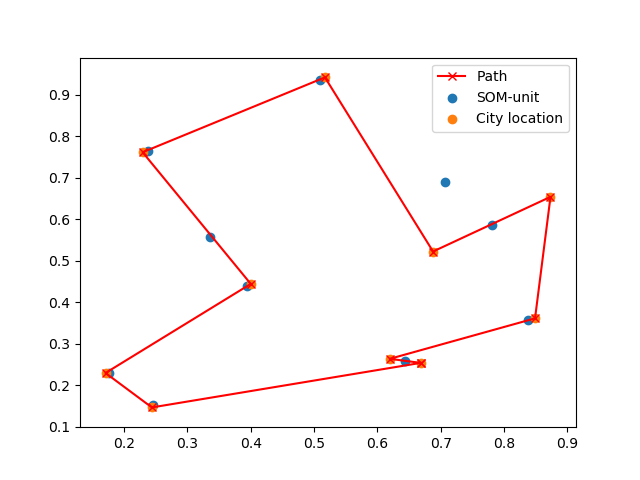
\includegraphics[width=\linewidth]{figures/cities1.png}
   \end{subfigure}
  \begin{subfigure}[b]{0.5\textwidth}
   \centering
   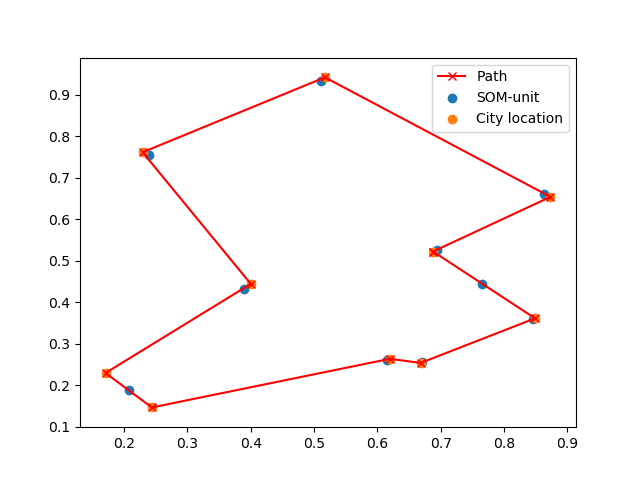
\includegraphics[width=\linewidth]{figures/cities2.png}
   \end{subfigure}
    \caption{Two different paths through the cities. Using the SOM-algorithm gives no guarantees of finding the absolute shortest route, however.}
   \label{fig:cities}
\end{figure}

In the case when one node is assigned as the closest node to multiple cities (i.e. some nodes are more or less 'dead'), the order in which these cities are visited become random. This may lead to suboptimal routes. 

\subsection{Clustering with SOM}

The SOM-algorithm was also implemented for a clustering task. This task involved ordering the votes of MPs in the Riksdag according to party, gender and district. The weight matrix was constructed as a vectorized version of a 10x10 grid. The members of the Riksdag were in total 349, each of which cast 31 votes. These votes were assigned the binary value of 0 for a 'no' and 1 for 'yes' (abstain/absence was given the value 0.5). Thus, the input space for each MP was mapped to an output grid of 10x10 through training by a SOM algorithm. The algorithm was initialized with a randomized weight matrix, and trained for 100 epochs with a learning rate of $\eta=0.2$, decaying by $0.99$ per epoch. The neighbourhood of the winning node was calculated through the Manhattan distance, and the update was applied to units within a distance function $D(t)$ as
\begin{align*}
  d = \vert x - x_\text{win} \vert + \vert y - y_\text{win}\vert < D(t)
\end{align*}
where $D(t) = 4 \exp{(-\frac{t^2}{\lambda})}$. This produced the mappings shown in Figures \ref{fig:parties}, \ref{fig:genders} and \ref{fig:districts}. It is possible to discern a classical right/left divide, with the right wing parties M and Kd mapped closer together. The centre parties Fp, C are mapped between the right and the left parties. S is closest to the centre parties, while the left wing parties V and Mp are mapped close together with the 'No party' MPs. There is some separation between male and female voters, with the male pattern similar to the 'No party' and the female pattern similar to 'M'. There is a large diversity in the MP voting patterns when sorting by district.


\begin{figure}[ht]
  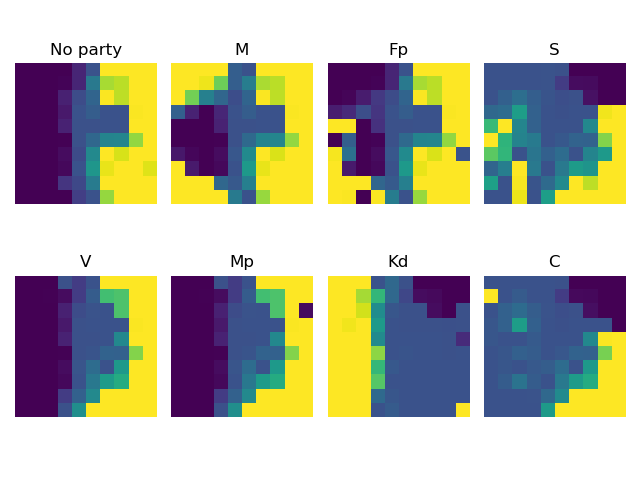
\includegraphics[width=\linewidth]{figures/parties.png}
  \caption{The clustering of voters according to party.}
    \label{fig:parties}
\end{figure}

\begin{figure}[ht]
  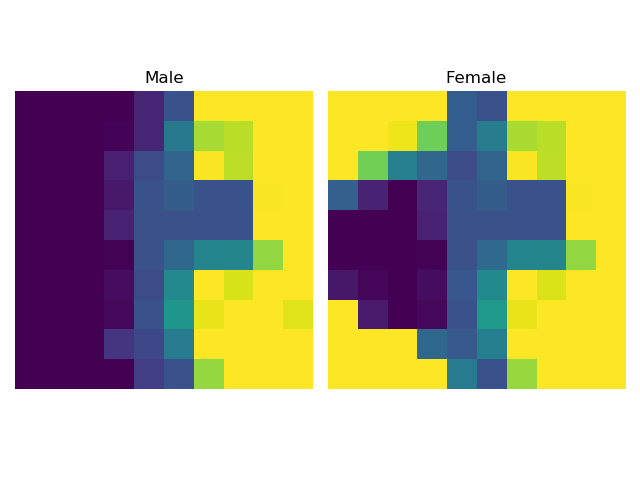
\includegraphics[width=\linewidth]{figures/genders.png}
  \caption{The clustering of voters according to gender.}
  \label{fig:genders}
\end{figure}

\begin{figure}[ht]
  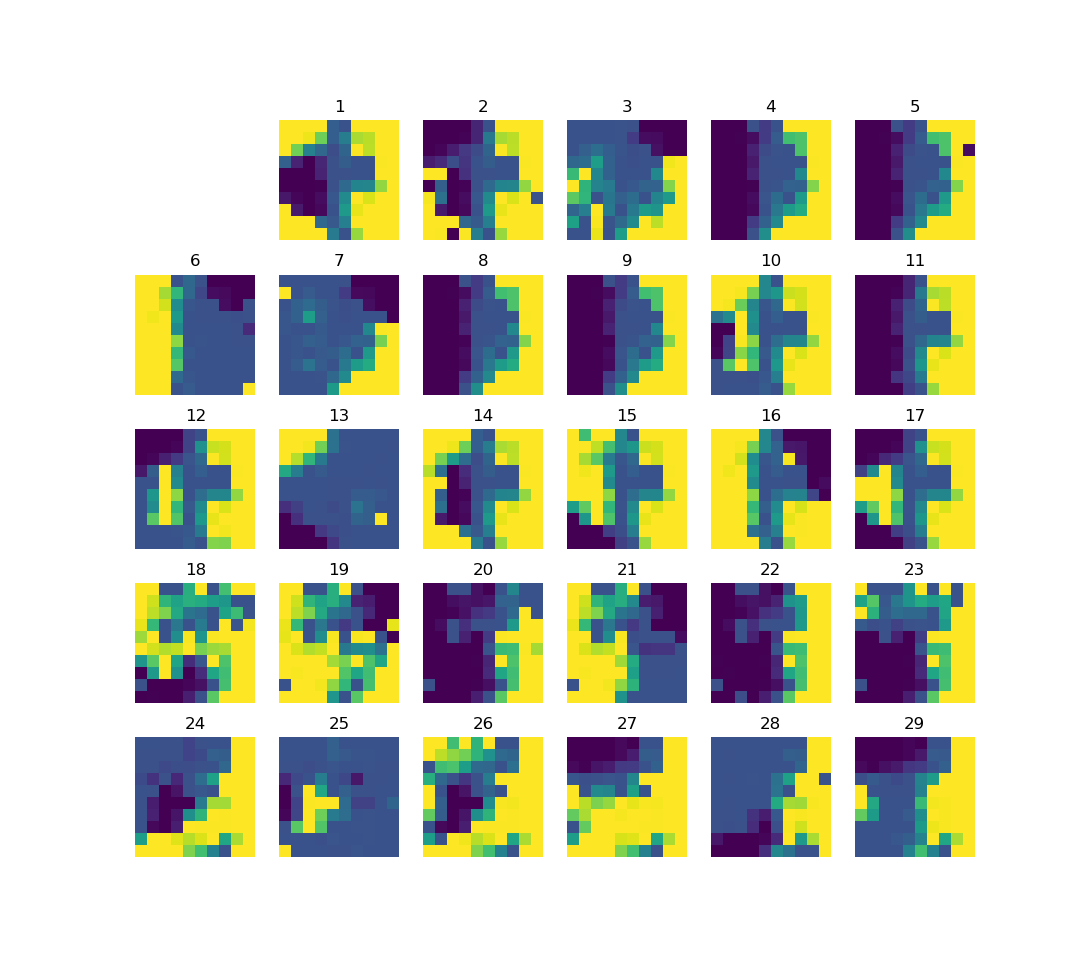
\includegraphics[width=\linewidth]{figures/districts.png}
  \caption{The clustering of voters according to district.}
  \label{fig:districts}
\end{figure}


\section{Final remarks \normalsize{\textit{(max 0.5 page)}}}

In this lab, I first implemented radial basis functions and their initialization through a simple competitive learning algorithm. The insights drawn from this competitive learning were then used to implement self organizing maps, a form of unsupervised learning, for a diverse set of datasets. The tasks were stimulating to solve, but required a lot of tinkering with hyperparameters (decay, learning rates, neighbourhoods et.c.) in order to get results that made sense. Figuring out how to map and calculate distances for 2-D grids was also a bit challenging.

\end{document}
